\providecommand{\main}{..}
\documentclass[\main/main.tex]{subfiles}
\begin{document}

Si tratta di un argomento legato all'apprendimento non supervisionato, che si occupa di raggruppare oggetti simili tra loro.

\begin{figure}[H]
  \centering
  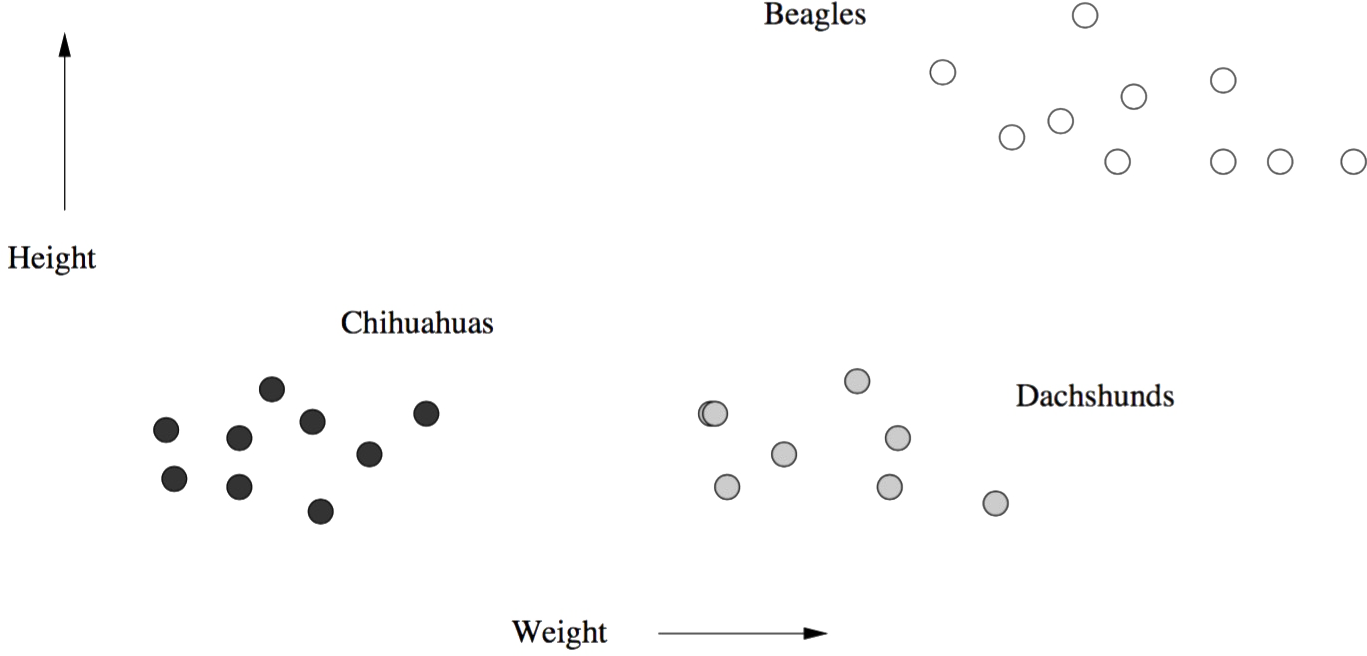
\includegraphics[width=0.75\textwidth]{dogs}
  \caption{Clustering di cani}
  \label{dog}
\end{figure}

\subsection{Esempio: clustering di cani}
Preso in considerazione per esempio uno spazio euclideo di 2 dimensioni, altezza e peso di alcuni cani. Viene considerato noto che le misurazioni siano solo di chihuhua, beagle e bassotti (Figura \ref{dog}).
Sicchè le zone sono ben identificate, potrebbe esserci una funzione tra altezza e peso, per esempio la razza del cane. Posso quindi dividere in 3 categorie, che posso utilizzare per classificare le razze di cane.

\section{The curse of dimensionality}
In uno spazio ad alta dimensione, la distanza euclidea tende a risultare costante. Inoltre, in uno spazio euclideo ad alta dimensione i vettori tendono ad essere normali tra loro.

\section{Approccio agglomerativo alla creazione di cluster}
Inizio costruendo un cluster per ogni punto e quindi procedo ad unire i cluster che io ritengo simili fra loro.

\begin{enumerate}
  \item Costruisco i cluster singoletti.
  \item while (!stop) $\{$
        \begin{enumerate}
          \item Scelgo due cluster
          \item Unisco i due cluster
        \end{enumerate}
  \item $\}$
\end{enumerate}

\begin{definition}[Centroide]
  Il baricentro dei punti di un cluster è detto \textbf{centroide} (figura \ref{centroids}) ed ha caratteristiche identificative di quel cluster.
  \begin{figure}[H]
    \centering
    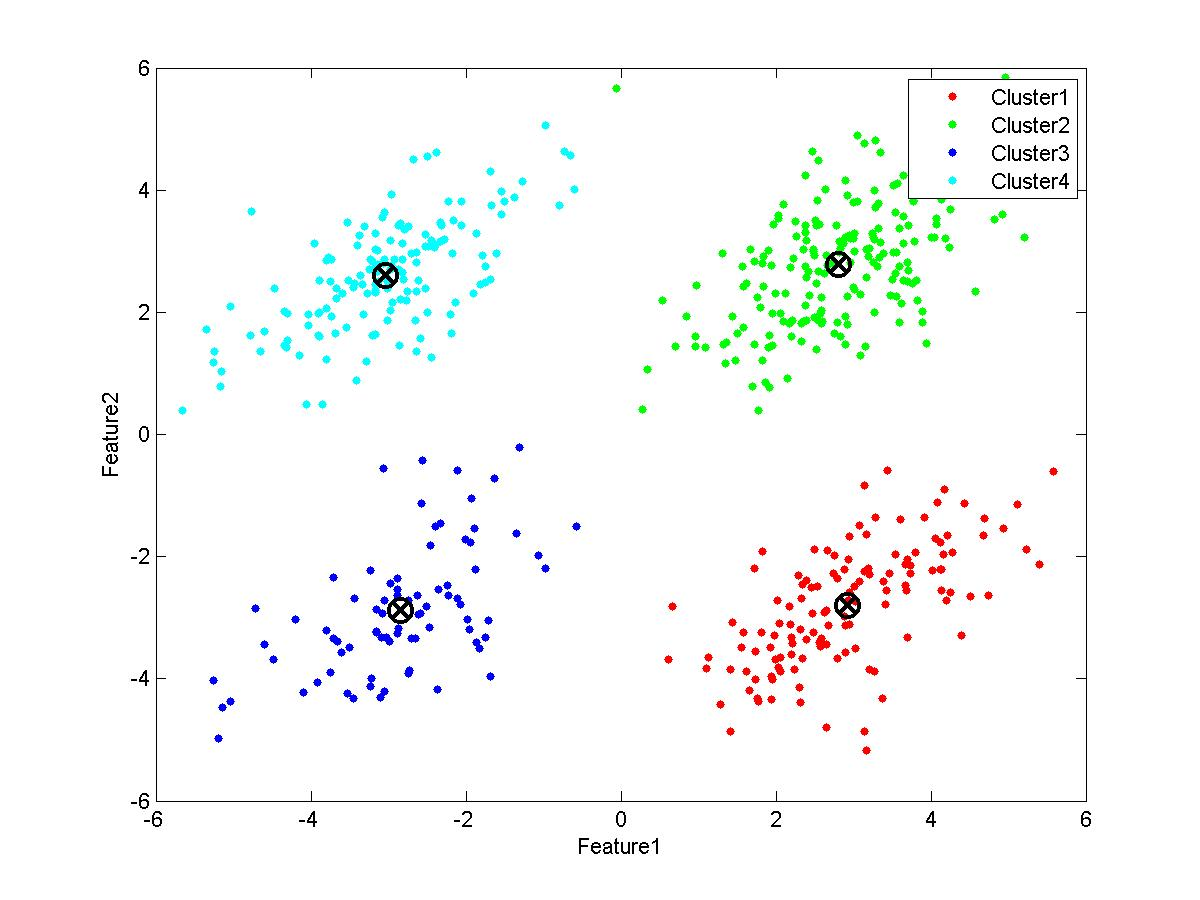
\includegraphics[width=0.5\textwidth]{centroid}
    \caption{Centroidi}
    \label{centroids}
  \end{figure}
\end{definition}

\begin{definition}[Clustroide]
  Un clustroide è un punto rappresentativo del cluster che non coincide con il \textbf{centroide}.
\end{definition}

Una regola possibile per fondere due cluster è identificare i punti più vicini tra i due centroidi. Una volta fusi, si ridetermina il nuovo centroide.

\begin{enumerate}
  \item Scelgo due cluster vicini e li unisco.
  \item Ridetermino il centroide del nuovo cluster così ottenuto.
  \item Ripeto sino a che non determino che i custer sono sufficientemente grandi.
\end{enumerate}

Questo procedimento ha complessità $O(n^3)$.

\begin{definition}[Dendrogramma]
  Un dentrogramma (figura \ref{dendrogramma}) è un metodo grafico con cui rappresentare come i cluster si uniscono di iterazione in iterazione.
  \begin{figure}[H]
    \centering
    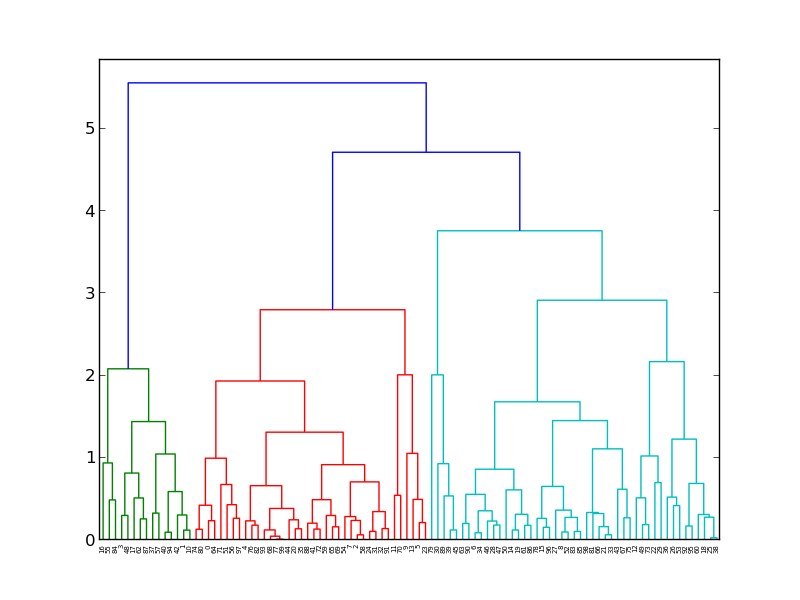
\includegraphics[width=0.5\textwidth]{dendrogram}
    \caption{Dendrogramma}
    \label{dendrogram}
  \end{figure}
\end{definition}

\subsection{Approccio agglomerativo a complessità computazionale ridotta}

\begin{enumerate}
  \item Calcolo la distanza tra $n^2$ coppie \dotfill \textbf{$O(n^2)$}
  \item Costruisco una coda di priorità tra gli elementi simili \dotfill \textbf{$O(n^2)$}
  \item \underline{Elimino le coppie dei cluster che fondo} \dotfill \textbf{$O(n\log n)$}
  \item \underline{Inserisco nelle coppire il nuovo cluster} \dotfill \textbf{$O(n\log n)$}
\end{enumerate}

La sezione \underline{iterative}, sottolineata nella lista, viene ripetuta $n$ volte, quindi la complessità computazionale risulta essere $O(n^2\log n)$.

\subsection{Quando fermare l'algoritmo?}
L'algoritmo viene interrotto quando i cluster diventano tropppo poco densi o il raggio del cluster troppo ampio (il raggio può essere calcolato sia dal centroide che dal clustroide).

\end{document}